% generated by make_figs.py -- do not edit by hand
\begin{figure*}[t]
\centering
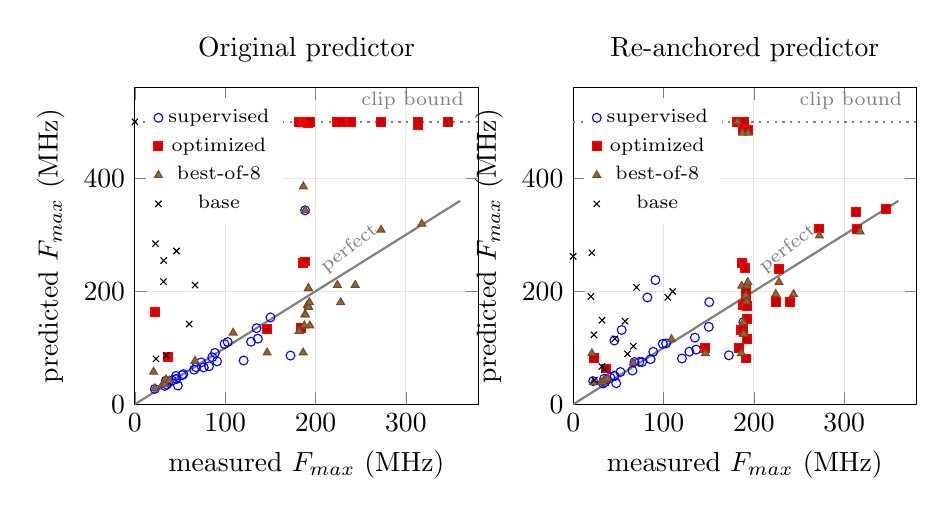
\begin{tikzpicture}

\begin{axis}[
  name=p0, title={Original predictor},
  width=.49\textwidth, height=5.6cm,
  xlabel={measured $F_{max}$ (MHz)}, ylabel={predicted $F_{max}$ (MHz)},
  xmin=0, xmax=380, ymin=0, ymax=560,
  legend pos=north west, legend style={font=\scriptsize, draw=none},
  grid=major, grid style={gray!20}
]
\addplot[gray, thick, domain=0:360, forget plot] {x};
\node[gray, font=\scriptsize, rotate=38, anchor=south] at (axis cs:250,250) {perfect};
\addplot[gray, dotted, thick, forget plot] coordinates {(0,500) (380,500)};
\node[gray, font=\scriptsize, anchor=south east] at (axis cs:375,505) {clip bound};
\addplot+[only marks, mark=o, mark size=1.6pt] coordinates {(22.1,27.1) (33.1,32.6) (34.3,41.8) (35.3,34.7) (37.1,38.6) (41.1,42.1) (45.6,44.8) (45.6,50.2) (45.9,44.7) (47.6,33.1) (52.3,51.4) (53.7,53.3) (65.6,61.2) (67.8,65.5) (73.3,74.1) (76.3,65.3) (82.1,67.3) (85.7,83.3) (88.6,90.9) (91.0,75.9) (99.2,106.7) (102.8,110.1) (120.4,77.5) (128.6,110.7) (134.7,134.7) (136.1,116.1) (150.1,153.7) (150.6,332.7) (172.3,86.2) (188.4,343.3)};
\addlegendentry{supervised}
\addplot+[only marks, mark=square*, mark size=1.6pt] coordinates {(22.8,162.6) (36.2,84.5) (146.4,133.3) (181.8,500.0) (183.9,134.7) (186.0,250.2) (186.5,500.0) (187.5,500.0) (188.1,252.7) (188.4,500.0) (189.6,500.0) (189.7,500.0) (191.1,500.0) (191.1,500.0) (191.1,500.0) (191.1,500.0) (191.1,500.0) (191.1,500.0) (191.2,500.0) (192.1,498.0) (192.1,500.0) (192.1,500.0) (193.7,500.0) (224.2,500.0) (227.8,500.0) (239.7,500.0) (272.5,500.0) (313.0,493.6) (313.7,500.0) (346.5,500.0)};
\addlegendentry{optimized}
\addplot+[only marks, mark=triangle*, mark size=1.6pt] coordinates {(20.7,57.4) (22.1,28.3) (30.6,35.2) (32.5,35.2) (32.6,35.2) (34.5,44.0) (38.1,41.8) (66.6,76.6) (108.8,126.6) (146.4,91.5) (181.8,129.4) (186.3,91.5) (186.5,385.4) (187.5,139.4) (188.1,158.5) (188.4,343.3) (188.9,158.5) (191.1,175.5) (191.1,175.5) (192.1,172.0) (192.1,172.0) (192.1,205.2) (192.1,205.2) (193.2,180.4) (193.7,139.4) (224.2,211.0) (227.8,180.4) (243.9,211.0) (272.5,308.8) (317.6,319.3)};
\addlegendentry{best-of-8}
\addplot+[only marks, mark=x, mark size=1.6pt] coordinates {(0.0,500.0) (19.6,500.0) (20.7,500.0) (22.9,284.3) (23.4,80.3) (29.8,500.0) (31.7,217.1) (31.9,254.4) (34.6,86.4) (46.1,271.3) (57.5,449.5) (60.1,141.9) (66.6,211.0) (70.1,405.7) (104.7,421.0) (110.1,444.5)};
\addlegendentry{base}
\end{axis}
\begin{axis}[
  at={(p0.right of south east)}, xshift=12mm, ylabel={}, title={Re-anchored predictor},
  width=.49\textwidth, height=5.6cm,
  xlabel={measured $F_{max}$ (MHz)}, ylabel={predicted $F_{max}$ (MHz)},
  xmin=0, xmax=380, ymin=0, ymax=560,
  legend pos=north west, legend style={font=\scriptsize, draw=none},
  grid=major, grid style={gray!20}
]
\addplot[gray, thick, domain=0:360, forget plot] {x};
\node[gray, font=\scriptsize, rotate=38, anchor=south] at (axis cs:250,250) {perfect};
\addplot[gray, dotted, thick, forget plot] coordinates {(0,500) (380,500)};
\node[gray, font=\scriptsize, anchor=south east] at (axis cs:375,505) {clip bound};
\addplot+[only marks, mark=o, mark size=1.6pt] coordinates {(22.1,41.0) (33.1,36.8) (34.3,45.2) (35.3,39.0) (37.1,43.7) (41.1,47.3) (45.6,50.1) (45.6,112.8) (45.9,50.1) (47.6,37.2) (52.3,57.1) (53.7,131.5) (65.6,59.7) (67.8,74.9) (73.3,75.1) (76.3,74.8) (82.1,189.0) (85.7,79.8) (88.6,92.8) (91.0,219.8) (99.2,106.9) (102.8,107.7) (120.4,81.1) (128.6,93.2) (134.7,117.9) (136.1,96.8) (150.1,137.1) (150.6,180.8) (172.3,86.7) (188.4,145.4)};
\addlegendentry{supervised}
\addplot+[only marks, mark=square*, mark size=1.6pt] coordinates {(22.8,82.4) (36.2,63.3) (146.4,99.1) (181.8,500.0) (183.9,99.6) (186.0,130.9) (186.5,249.5) (187.5,484.6) (188.1,131.8) (188.4,176.2) (189.6,500.0) (189.7,240.8) (191.1,188.1) (191.1,192.6) (191.1,194.4) (191.1,201.8) (191.1,202.5) (191.1,201.6) (191.2,81.0) (192.1,116.0) (192.1,150.6) (192.1,173.6) (193.7,484.6) (224.2,180.9) (227.8,239.4) (239.7,180.2) (272.5,311.1) (313.0,340.5) (313.7,310.6) (346.5,345.4)};
\addlegendentry{optimized}
\addplot+[only marks, mark=triangle*, mark size=1.6pt] coordinates {(20.7,90.1) (22.1,38.6) (30.6,39.0) (32.5,39.0) (32.6,39.0) (34.5,42.5) (38.1,45.2) (66.6,73.5) (108.8,115.1) (146.4,90.2) (181.8,500.0) (186.3,90.2) (186.5,209.4) (187.5,480.2) (188.1,124.3) (188.4,145.4) (188.9,124.3) (191.1,192.1) (191.1,192.1) (192.1,181.6) (192.1,181.6) (192.1,209.9) (192.1,209.9) (193.2,216.1) (193.7,480.2) (224.2,195.0) (227.8,216.1) (243.9,195.0) (272.5,298.4) (317.6,305.8)};
\addlegendentry{best-of-8}
\addplot+[only marks, mark=x, mark size=1.6pt] coordinates {(0.0,261.9) (19.6,190.7) (20.7,268.1) (22.9,122.9) (23.4,42.8) (29.8,500.0) (31.7,66.9) (31.9,148.8) (34.6,61.6) (46.1,115.9) (57.5,146.9) (60.1,89.2) (66.6,102.7) (70.1,206.9) (104.7,189.3) (110.1,199.7)};
\addlegendentry{base}
\end{axis}
\end{tikzpicture}
\caption{Predicted against measured \fmax{} for every (policy, design) cell of
the held-out set, both count-weighted. Left: the original predictor. Supervised
and best-of-8 cells sit on the identity line; the optimized policy's cells lift
off it and pile against the reward's clip bound, where the reward can no longer
order one design against another. Right: the same candidates under the
re-anchored predictor. The correction is specific to the region optimisation
created, and the supervised cells are unaffected.}
\label{fig:scatter}
\end{figure*}
